\documentclass{xStandalone}

\begin{document}
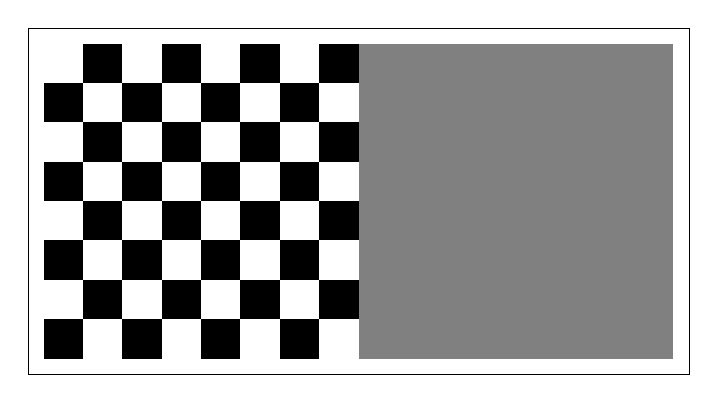
\begin{tikzpicture}

\def\step{0.5}
\foreach \x in {0,\fpeval{\step*2},...,3.99}
{
    \foreach \y in {0,\fpeval{\step*2},...,3.99}
    {
        \fill[black] (\x,\y) rectangle (\fpeval{\x+\step},\fpeval{\y+\step});
        \fill[black] (\fpeval{\x+\step},\fpeval{\y+\step}) rectangle (\fpeval{\x+2*\step},\fpeval{\y+2*\step});
    }
}

\fill[white!\fpeval{100*0.5}!black] (4,0) rectangle (8,4);

\draw[ultra thin] (-0.2,-0.2) rectangle (8.2,4.2);

\end{tikzpicture}
\end{document}